\documentclass[12pt]{article}

\usepackage{mathtools}
\usepackage{fontspec}
\usepackage{unicode-math}
\setmainfont{STIX Two Text}
\setsansfont{TeX Gyre Heros}
\setmathfont{STIX Two Math}

\usepackage[margin=1.25in]{geometry}
\usepackage{setspace}
\setstretch{1.08}
\usepackage{textcomp}
\usepackage{microtype}
\usepackage{enumitem}
\usepackage{tabularx}
\usepackage{booktabs}
\usepackage{array}
\newcolumntype{R}{>{\raggedleft\arraybackslash}X}
\usepackage{multirow}

\usepackage{graphicx}
\usepackage[font=small,labelfont=bf]{caption}

\usepackage{amsmath}
\usepackage{amsfonts}
\usepackage{diffcoeff}

\usepackage{hyperref}
\usepackage{cleveref}
\usepackage{natbib}

\newcommand{\Ecar}{E^\text{car}}
\newcommand{\Etransit}{E^\text{transit}}
\newcommand{\Ecordon}{E^\text{cordon}}
\newcommand{\W}{\mathcal{W}}
\newcommand{\Pset}{\mathcal{P}}
\newcommand{\POD}{\Pset_{od}}
\newcommand{\PcarOD}{\Pset_{od}^\text{car}}
\newcommand{\PtransitOD}{\Pset_{od}^\text{transit}}
\newcommand{\set}[2]{\left\{\,#1 \;\middle|\; #2\,\right\}}
\newcommand{\R}{\mathbb{R}}
\newcommand{\Rp}{\R_{+}}
\renewcommand{\vec}[1]{\mathbf{#1}}

\DeclarePairedDelimiter{\abs}{\lvert}{\rvert}
\DeclarePairedDelimiter{\norm}{\lVert}{\rVert}
\DeclareMathOperator{\TSC}{TSC}

\let\epsilon\varepsilon

\title{Stochastic User Equilibrium and System Optimum in Congested Transportation Networks}
\author{Eric Ordonez}
\date{May 8, 2026}
\makeatletter
\hypersetup{
	pdftitle={\@title},
	pdfauthor={\@author}
}
\makeatother

\begin{document}

\maketitle

\begin{abstract}
    We study the efficiency of congestion pricing policies in a transportation network model with stochastic route choice.
    Using a logit-based stochastic user equilibrium, we compare system-optimal flows with decentralized equilibria under edge-based tolling and cordon tolling schemes.
    We evaluate welfare loss and mode share as functions of toll levels and behavioral responsiveness.
    We find that while optimal tolling can closely approximate the system optimum, second-best policies are sensitive to traveler responsiveness and network structure.
\end{abstract}

\section{Introduction}

Traffic congestion is a defining inefficiency of modern cities.
The welfare economics interpretation of this inefficiency views travelers as users of a transportation network who choose their routes independently of others.
They account only for their own travel time while ignoring the delays imposed on others. 
This difference between private and social cost generates congestion as a negative externality of individual decision making \citep{pigou1920welfare}.
Left unchecked, its consequences have long been manifest in major cities; it is well understood that unconstrained road use generally leads to inefficient overutilization \citep{knight1924socialcost}.

Congestion pricing set in response to the marginal costs of the externality can decentralize the socially efficient traffic allocation \citep{vickrey1969congestion}.
That is, the welfare losses due to congestion can be recovered by a pricing structure that incentivizes travelers to reroute and thereby redistribute the congestion.
Modern policies implementing this theory include London's flat daily charge for driving into central London and New York City's variable rate toll to drive into downtown Manhattan.

This project studies how such pricing policies affect traffic flows, social welfare, and transportation mode choice in a stylized urban setting.
We construct a multiplex transportation network in which travelers choose among car and transit routes according to a stochastic discrete choice model.
Road travel times depend on congestion through flow-dependent link costs, while transit provides a fixed-cost alternative.
Individual route choices generate network flows, which in turn determine travel costs, producing a stochastic user equilibrium.

Using this framework, we compare three pricing regimes: an unpriced equilibrium, first-best marginal-cost pricing, and second-best cordon pricing.
Simulations are performed across three stylized urban network topologies.
Particular attention is given to behavioral heterogeneity through route-choice sensitivity, which governs how strongly travelers respond to differences in travel times and costs.

\section{Model}

\subsection{Network structure}

We consider a city with two modes of transportation: cars and transit.
The transportation network is a multiplex directed graph $G = (V, \Ecar, \Etransit)$ consisting of a road network $\Ecar$ and transit network $\Etransit$.
The shared nodes $V$ represent major street intersections, hubs, and stations; the edges $E = \Ecar \cup \Etransit$ represent routes between them.
$\Etransit$ is not necessarily a subset of $\Ecar$; in practice, it is sparser.
We assume that everywhere reachable by transit is also reachable by car and that there are many more routes available by car.

An origin-destination (OD) pair of nodes is connected through both layers via feasible paths.
Let $\W$ be the set of all OD pairs, and for each $(o, d) \in \W$, let $\PcarOD$ and $\PtransitOD$ denote the sets of car paths and transit paths, respectively, from $o$ to $d$.
Each OD pair carries a fixed demand $q_{od} > 0$.
This represents people that need to travel from one location to another for reasons exogenous to the network and model.

We are primarily concerned with flow through the network, which we represent with edge weights.
For all edges $e \in E$, the edge flow $x_e \geq 0$ is the average rate of users traversing edge $e$ over a given time interval.
For a road edge, this is interpreted as the average number of vehicles; for transit edges, it is passenger flow.

For any path $p$, the path flow $f_p$ is interpreted as the average rate of choosing path $p$.
It is a model primitive that induces edge flows, $x_e$, by
\begin{equation}
    \label{eqn:conservation_of_flow}
    x_e = \sum_{(o, d) \in \W} \sum_{p \in \POD} \delta_{ep} f_p, \quad \text{where }
    \delta_{ep} =
    \begin{cases}
        1 &\text{if } e \in p, \\
        0 &\text{otherwise.}
    \end{cases}
\end{equation}
We require that edge flows and path flows be mutually consistent in that a path flow equals the sum of the flows of its constituent edges, and that the conservation of flow in \Cref{eqn:conservation_of_flow} holds for all edges.
Implicitly, this means that $\W$ specifies the total path flow in the network.
Finally, let $\vec{x}$ denote the vector of all edge flows and $\vec{f}$ the vector of all path flows $f_p$ for all $p \in \bigcup \set{\POD}{(o, d) \in \W} =: \Pset$.
This is mostly for notational convenience.

The key difference between car and transit routes is in their user costs, which determines which paths are chosen and how travelers flow through the network. 
Path costs depend on edge flows, edge flows depend on path flows, and path flows depend on path costs.
We now impose a cost structure that allows this circular dependency to admit a system equilibrium.

\subsection{Cost structure}

Cost is an abstract, user-perceived measurement that combines travel time and price.
Users of the network assess the costs of paths to decide which one, and consequently which mode, to take.

First, consider road edges $e \in \Ecar$.
These are subject to congestion, which increases the time to take that route.
The actual travel time $t_e$ is a function of the edge flow $x_e$, and we model this with the BPR function:\footnote{The Bureau of Public Roads (BPR) function is a volume-delay function that deterministically maps traffic volume to travel time on a network link. It is the most widely used volume-delay function in static traffic assignment models.}
\[
    t_e(x_e) = t_e^0 \left[1 + \alpha \left(\frac{x_e}{K_e}\right)^\beta\right].
\]
Each edge has a fixed capacity $K_e$ and a free-flow travel time $t_e^0$.
The capacity represents the maximum flow that the road is designed for\footnote{This means that $K$ is not a hard upper limit. Flows greater than $K$ can be considered heavy congestion.}, and $t_e^0$ represents the time it takes to traverse $e$ in the absence of congestion.
$\alpha$ and $\beta$ are scale and shape parameters, respectively; we assume they are homogenous across the network, i.e., the same for all road edges.

We introduce congestion pricing as a toll $\tau_e(x_e) \geq 0$ set on each road edge by a social planner in response to congestion \citep{vickrey1969congestion}.
For simplicity, let road edge cost be the sum of flow-induced travel time and the toll:
\[
    c_e(x_e) = t_e(x_e) + \tau_e(x_e).
\]
We also assume that edge costs are additive so that path cost equals the sum of the costs of its component edges.
Thus, for any path $p \in \PcarOD$, its user cost is
\[
    C_p(\vec{x}) = \sum_{e \in p}{c_e(x_e)} = \sum_{e \in p}{t_e(x_e) + \tau_e(x_e)}.
\]

For tractability, we assume that only car routes are congestible.
This is not completely unrealistic, depending on the transit network. 
Since cars comprise the vast majority of road congestion, non-congestible transit routes can make sense if they can operate independently of cars on the road, like dedicated bus lanes or subway lines.
This is still, of course, an oversimplification that could be addressed by disaggregating transit modes by susceptibility to congestion, e.g., buses vs.\ subways, or by incorporating transit capacity.

Transit paths do not depend on congestion, but we suppose a fixed price $\kappa > 0$ for using them.
Note that this cost is imposed on the path and not on individual edges.
This captures the idea that transit usage is not free like car usage is implicitly assumed to be.
It also reflects paying a single fare for transit regardless of distance traveled.

Instead, all transit edges $e \in \Etransit$ have a fixed travel time $\overline{t}$, as we assume there is no congestion.
This quantity also captures the average time spent waiting for and transferring on transit.
This gives transit edges the constant cost
\[
    c_{e}(x_{e}) = \overline{t}
\]
so that for any $p \in \PtransitOD$, its user cost is 
\[
    C_p(\vec{x}) = \sum_{e \in p}{c_{e}(x_{e})} + \kappa = \overline{t} \cdot \abs{p} + \kappa.
\]
Note that transit path cost is independent of $\vec{x}$.
So it need not be denoted $C_p(\vec{x})$, but we do so for notational convenience in the discrete choice model and stochastic user equilibrium that follow.

% Wardrop equilibrium (WIP)
\subsection{Deterministic user equilibrium}

Under deterministic route choice, travelers select the minimum-cost path from $o$ to $d$.
A user equilibrium \citep{wardrop1952traffic} is a feasible flow such that for each $(o, d) \in \mathcal{W}$, all used paths have equal and minimal cost, while unused paths have weakly higher cost.

Equivalently, $\vec{x}^\ast$ is a deterministic user equilibrium if for all $p, p' \in \POD$, if $f_p > 0$, then
\[
    C_p(\vec{x}^\ast) \leq C_{p'}(\vec{x}^\ast)
\]
for all $p' \in \POD$.
This is also called a Wardrop equilibrium.

% Wardrop equilibrium (WIP)

\subsection{Discrete choice over paths}

Given these perceived path costs, travelers choose their route, and consequently their mode, according to a discrete choice model. 
Each OD pair $(o, d)$ splits across all paths in $\POD = \PcarOD \cup \PtransitOD$.
At the individual level, each traveler going from $o$ to $d$ chooses exactly one path given all edge flows $\vec{x}$. 
In this model, these individual, discrete decisions are made according to a random utility framework \citep{mcfadden1974logit} and aggregated into probabilistic flows.

For each path $p \in \POD$, the utility to a traveler is given by
\[
    U_p = -C_p(\vec{x}) + \epsilon_p,
\]
where $C_p(\vec{x})$ is the user-perceived cost of path $p$ and $\epsilon_p$ is a random utility shock.
Intuitively, travelers seek to maximize their utility by minimizing the expected cost.
We assume that the shocks $\{\epsilon_p\}$ are independent and identically distributed according to a Gumbel distribution \citep{mcfadden1974logit}.
Under this assumption, the probability that a traveler selects path $p$ is given by the logit model
\[
    \Pr{(p)} = \frac{\exp{(-\theta C_p(\vec{x}))}}{\sum_{p' \in \POD}{\exp{(-\theta C_{p'}(\vec{x}))}}}
\]
where $\theta > 0$ is a parameter governing sensitivity to cost differences.
Aggregating over the total demand $q_{od}$, the induced flow on path $p$ is
\begin{equation}
    \label{eqn:single_logit_model}
    f_p = q_{od} \cdot \frac{\exp{(-\theta C_p(\vec{x}))}}{\sum_{p' \in \POD}{\exp{(-\theta C_{p'}(\vec{x}))}}}
\end{equation}

This formulation implies that travelers probabilistically choose among all available car and transit routes, with lower-cost paths receiving higher flow.
The parameter $\theta$ controls the degree of responsiveness: as $\theta \to \infty$, travelers increasingly concentrate on minimum-cost paths, while for small $\theta$, choices become more diffuse.

Importantly, path costs for car routes depend on congestion through edge flows, while path flows are determined by these same costs.
As a result, the model defines a coupled system in which flows and costs must be determined simultaneously.
The resulting equilibrium is characterized as a fixed point of the mapping from path costs to path flows.

\subsection{Stochastic user equilibrium}

Define the logit assignment operator $\Lambda: \Rp^{\abs{E}} \rightarrow \Rp^{\abs{\Pset}}$ by
\[
    \left[\Lambda(\vec{x})\right]_p = q_{od} \cdot \frac{\exp{(-\theta C_p(\vec{x}))}}{\sum_{p' \in \POD}{\exp{(-\theta C_{p'}(\vec{x}))}}}, \quad p \in \POD
\]
and the edge flow aggregation operator $\Phi: \Rp^{\abs{\Pset}} \rightarrow \Rp^{\abs{E}}$ by
\[
    \left[\Phi(\vec{f})\right]_e = \sum_{(o, d) \in \W} \sum_{p \in \POD} \delta_{ep} f_p.
\]
A stochastic user equilibrium (SUE) \citep{wardrop1952traffic,daganzo1977stochastic} is a fixed point $\vec{x}^\ast$ of the composition $\Psi = \Phi \circ \Lambda$:
\[
    \vec{x}^\ast = \Psi(\vec{x}^\ast) = \Phi(\Lambda(\vec{x}^\ast)).
\]
In this network, a SUE is a vector of path flows $\vec{f}^\ast$ (and corresponding vector of edge flows $\vec{x}^\ast$) such that for every $(o, d) \in \W$ and every $p \in \POD$:
\begin{itemize}[noitemsep]
    \item $x_e^\ast$ satisfies the conservation of flow (\Cref{eqn:conservation_of_flow}) for all $e \in E$.
    \item The induced path flow $f_p^\ast$ equals the demand $q_{od}$ (\Cref{eqn:single_logit_model}).
\end{itemize}

To prove the SUE's existence, recall that edge flows are nonnegative and bounded.
So the feasible flow set
\[
    \set{\vec{x} \geq \vec{0}}{\sum_{e \in E} x_e \leq \sum_{(o,d) \in \W} q_{od}} \subset \Rp^{\abs{E}}
\]
is compact, as total demand is finite and each path is finite.
$\Psi$ is continuous because it is the composition of continuous functions, and it maps $\Rp^{\abs{E}}$ to itself.
Thus, by Brouwer's fixed-point theorem, there exists a point $\vec{x}^\ast \in \Rp^{\abs{E}}$ such that $\Psi(\vec{x}^\ast) = \vec{x}^\ast$.

Uniqueness is not necessarily guaranteed under the logit choice model.
Under continuous and strictly increasing road costs, which we have under the BPR formulation, the equilibrium is at least well-posed.
In practice, fixed-point iteration converges to a stable solution in our simulations, and we will refer to it as the SUE for simplicity.

\subsection{The social planner's problem}

The SUE characterizes the decentralized equilibrium outcome under individual utility maximization.
We now contrast this with the centralized outcome that a social planner would implement.

\subsubsection{Unpriced benchmark}

Define total social cost (TSC) as the sum of all travel costs in the network:
\[
    \TSC(\vec{x}) = \sum_{e \in E} x_e c_e(x_e)
\]
Recall that $\kappa$ is a path-level transit cost that factors in users' individual decisions, but it does not appear in the edge-level definition of TSC.
If we interpret $\kappa$ as a transit fare, we treat it as a transfer rather than a resource cost, so it is excluded from social cost.

The social planner seeks to solve
\[
    \min_{\vec{f} \geq \vec{0}}{\TSC(\vec{x}(\vec{f}))} = \min_{\vec{f} \geq \vec{0}}{\sum_{e \in E} x_e c_e(x_e)}
\]
subject to flow conservation constraints.
This is the classical network assignment framework \citep{dafermos1969assignment}.

The key distinction from the user's problem is that $x_e c_e(x_e)$ is the total cost borne by all users on edge $e$, not the average cost $c_e(x_e)$ experienced by a single user.
The planner interalizes the congestion externality \citep{knight1924socialcost}.
Adding one unit of flow to $e$ increases the cost for all users on $e$ by $x_e c_e'(x_e)$, a cost that the individual user ignores because he does not internalize the externality.

The gap between social and user marginal cost is
\begin{align*}
    \mathrm{MSC}_e - \mathrm{MUC}_e &= \diff{}{x_e} x_e c_e(x_e) - \diff{}{x_e} c_e(x_e) \\
    &= \left(x_e c_e'(x_e) + c_e(x_e)\right) - c_e(x_e) \\
    &= x_e c_e'(x_e) \\
    &> 0,
\end{align*}
which is strictly positive under the BPR formulation for $c_e$.
The SUE, therefore, is generally inefficient; it overloads congested road edges relative to the social optimum.

\subsubsection{First-best edge tolling}

The planner can decentralize the social optimum by imposing a Pigouvian toll\footnote{A Pigouvian tax is a tax imposed on activities that generate negative externalities.} $\tau^\ast$ on each road edge $e$ equal to the marginal congestion externality evaluated at the optimal flow $x_e^\ast$ \citep{vickrey1969congestion}:
\[
    \tau_e^\ast(x_e^\ast) = x_e^\ast c_e'(x_e^\ast).
\]
Under BPR, we get the closed form
\[
    c_e'(x_e^\ast) = t_e^0 \cdot \frac{\alpha \beta}{K_e} \left(\frac{x_e^\ast}{K_e}\right)^{\beta - 1}
\]
so that the first-best toll is
\[
    \tau_e^\ast(x_e^\ast) = t_e^0 \cdot \frac{\alpha \beta x_e^\ast}{K_e} \left(\frac{x_e^\ast}{K_e}\right)^{\beta - 1}.
\]
When users face the toll-inclusive cost $c_e(x_e) + \tau_e^\ast(x_e) = \mathrm{MSC}_e$, the resulting SUE replicates the social optimum \citep{pigou1920welfare,knight1924socialcost,vickrey1969congestion}.
In practice, implementing the differentiated per-edge tolls across an entire network is administratively and politically infeasible, which motivates a second-best solution via cordon tolling.

\subsubsection{Second-best cordon tolling}

A cordon toll imposes a fixed charge $\overline{\tau} > 0$ on road edges entering a designated zone $Z \subset V$, with all other road edge tolls set to zero.
Formally, let
\[
    \Ecordon = \set{(u, v) \in \Ecar}{u \notin Z, v \in Z}
\]
be the set of cordon-entering edges.
The toll structure is
\[
    \tau_e =
    \begin{cases}
        \overline{\tau} &\text{if } e \in \Ecordon, \\
        0 &\text{otherwise.}
    \end{cases}
\]
This is a second-best instrument.
It approximates the first-best by targeting the most congested zone, but it cannot replicate it because it applies a uniform toll rather than differentiated edge-level tolls.

The optimal second-best cordon toll solves a bilevel program.
The planner minimizes TSC at the upper level, anticipating the SUE response at the lower level, and this is generally nonconvex and computationally intensive.

Instead, in this project we evaluate cordon tolling as a fixed congestion pricing policy.
We set $\overline{\tau}$ equal to the average first-best toll on cordon-entering edges under the unpriced SUE, impose it and recompute the equilibrium, and compare welfare outcomes with the unpriced and first-best benchmarks.
This reflects how cordon schemes are implemented in practice in cities such as London and New York City, where a fixed fee schedule is set administratively rather than continuously optimized.

\section{Simulation}

\subsection{Network topologies}

To evaluate the pricing policies across different urban structures, we consider three stylized network topologies that resemble realistic city layouts where congestion pricing could be applied.
Each network features different connectivity patterns designed to capture distinct forms of urban organization.
They are visualized in \Cref{fig:stylized_networks} and are as follows:
\begin{enumerate}[noitemsep]
    \item \textbf{Grid network:} Manhattan-style urban traffic with many alternative routes and diffuse congestion.
    \item \textbf{Hub-and-spoke network:} A commuter rail-style city where congestion concentrates near a central hub.
    \item \textbf{Core-periphery network:} Suburban-style commuting with a dense downtown core and an outer ring transit service.
\end{enumerate}
\begin{figure}[htbp]
    \centering
    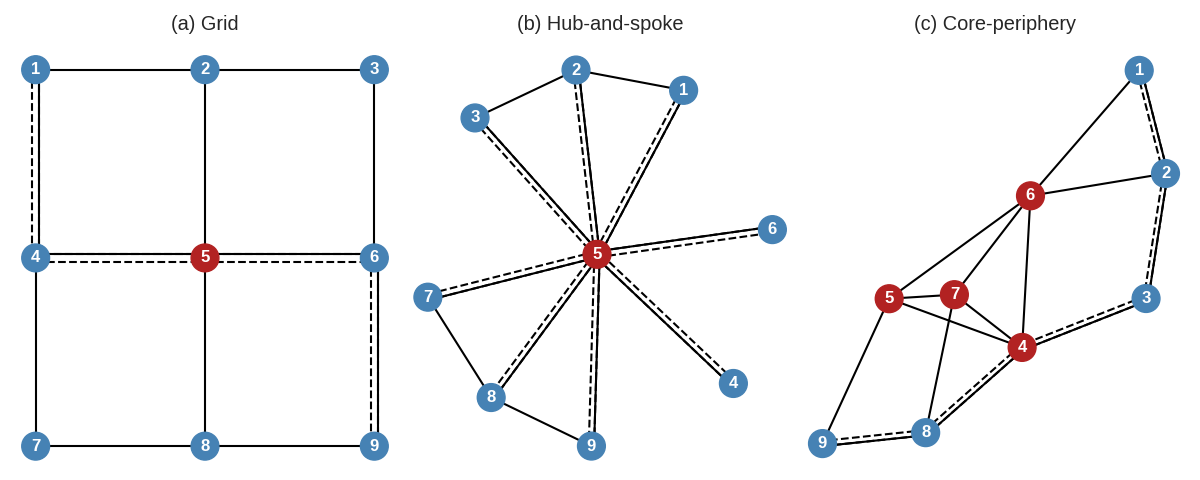
\includegraphics[width=\linewidth]{images/network_topologies.png}
    \caption{Three stylized networks. Cordon zone nodes $Z$ are colored red. The solid lines are road connections; the dashed lines, transit.}
    \label{fig:stylized_networks}
\end{figure}
In reality, these topologies are not mutually exclusive nor completely descriptive of any city.
A real city can exhibit features of all three topologies and more.

\subsection{Parameters}

All simulations use a common set of baseline parameters.
The BPR function parameters are set to the standard values $\alpha = 0.15$ and $\beta = 4$, following the original Bureau of Public Roads specification.
The fixed transit cost is $\kappa = 0.5$, and the baseline sensitivity is $\theta = 1$ with later robustness checks at $\theta = 0.5$ and $\theta = 2$.

Road edge parameters differ both within and across networks to reflect road hierarchies and layouts.
\begin{itemize}[noitemsep]
    \item \textbf{Grid:} The edges passing through the core are meant to represent the spine of the city, so they have higher capacity ($t_0 = 2$, $K = 15$) than the peripheral edges ($t_0 = 2$, $K = 10$).
    Transit is in general faster ($\overline{t} = 1.5$).
    
    \item \textbf{Hub-and-spoke:} The spokes offer an equal travel time to the hub ($t_0 = 3$, $K = 10$; $\overline{t} = 3$).
    Road travel in the periphery is faster but not as high-capacity ($t_0 = 2, K = 8$).
    
    \item \textbf{Core-periphery:} Connector roads link the periphery to the core ($t_0 = 2$, $K = 10$), but that travel is not any faster than within the periphery ($t_0 = 2$, $K = 10$).
    The core is dense $(t_0 = 1$, $K = 12$).
    Transit in the outer ring is generally faster than cars because it avoids the core ($\overline{t} = 1.5$).
\end{itemize}
(See the code repository for the specific edges to which these descriptions apply.)
Like the network topologies, note that these are stylized values and not empirically calibrated.

Each network's set of OD pairs, $\mathcal{W}$, is chosen to balance cordon crossing with peripheral travel, as well as to keep the number of feasible paths manageable, which is around 30.
(See the code repository for the exact pairs.)
Given an OD pair $(u, v)$, feasible paths are generated by finding all paths from $u$ to $v$ and dropping any car path longer than 4 and any transit path longer than 7.

Given $\mathcal{W}$ for each network, we calibrate aggregate demand as follows.
We sweep over a range of $q$ values and set $q_{od} = q$ for each OD pair.
Then we solve for the SUE and compute the maximum road saturation in the network, $\max_{e \in \Ecar}{x_e/K_e}$.
We target a $q$ such that the maximum saturation is approximately 1; this induces flows such that the network at baseline is already suffering from congestion.
This process yielded $q_{od}^\text{grid} = 6.52$, $q_{od}^\text{hub} = 9.34$, and $q_{od}^\text{core} = 5.55$.

\subsection{Experiments}

We conduct two sets of experiments.
The first evaluates the three congestion pricing regimes (unpriced, first-best edge tolling, and second-best cordon tolling) across each of the three network topologies.
We compute the SUE via fixed-point iteration, record the resulting mode shares and TSC, and visualize the SUE edge-level flows as heat maps colored by road saturation $x_e/K_e$.
The second experiment is a sensitivity analysis of the cost-sensitivity parameter $\theta$.
We repeat the first experiment with $\theta = 0.5$ and $\theta = 2.0$ but omit the heat maps.

We implement the following algorithm for fixed point iteration:
\begin{itemize}[noitemsep]
    \item Initialize $\vec{x}^{(0)} = \vec{0}$.
    \item Iterate $\vec{f}^{(k+1)} = \Lambda\left(\vec{x}^{(k)}\right)$ and $\vec{x}^{(k+1)} = \Phi\left(\vec{f}^{(k+1)}\right)$.
    \item Terminate if $\norm{\vec{x}^{(k+1)} - \vec{x}^{(k)}}_\infty < \varepsilon$.
\end{itemize}
For stability, we apply a damping weight $\eta \in (0, 1)$ to all new edge flows before checking for convergence in each iteration:
\[
    x_e^{(k+1)} \leftarrow  \eta x_e^{(k+1)} + (1 - \eta) x_e^{(k)}.
\]
We achieved convergence with $\eta = 0.5$.

For cordon tolling, the designated zone $Z$ is the set of nodes constituting the densely connected core of each network.
Specifically, this is node 5 in the grid and hub-and-spoke networks and nodes 4, 5, 6, and 7 in the core-periphery network.
The cordon toll is set equal to the average first-best Pigouvian toll on cordon-crossing edges evaluated at the unpriced SUE.

\section{Results}

\subsection{Mode shares}

\Cref{tab:mode_shares_baseline} reports equilibrium mode shares across the three networks and pricing regimes at the baseline $\theta = 1$.
In all cases, congestion pricing shifts demand from cars to transit, though the magnitude of this shift varies with the topology.
The hub-and-spoke network exhibits the most pronounced response: first-best pricing reduces the car share from 0.70 to 0.45, yielding a majority transit share that reflects the high road and transit connectedness of the hub.
The grid network produces a more moderate shift (0.80 to 0.69), consistent with the availability of alternative routes that diffuse congestion and mitigate the marginal cost of car travel.
The core-periphery network shows the smallest shift (0.88 to 0.81), suggesting that the lack of transit connections between the periphery and the core limits the competitiveness of transit for a large proportion of users.

Cordon tolling recovers a portion of the first-best mode shift in all three networks, but it falls short in each case.
The gap between cordon and first-best car shares is smallest in the hub-and-spoke network (0.65 vs.\ 0.45), where congestion is unavoidable because of how all major car routes must pass through the hub.

\begin{table}[htbp]
    \centering
    \footnotesize
    \begin{tabularx}{0.75\textwidth}{l l R R}
    \toprule
    \textbf{Network} & \textbf{Pricing} & \textbf{Car share} & \textbf{Transit share} \\
    \midrule
    Grid            & Unpriced   & $0.7978$ & $0.2022$ \\
                    & First-best & $0.6925$ & $0.3075$ \\
                    & Cordon     & $0.7714$ & $0.2286$ \\
    \midrule
    Hub-and-spoke   & Unpriced   & $0.7004$ & $0.2996$ \\
                    & First-best & $0.4526$ & $0.5474$ \\
                    & Cordon     & $0.6467$ & $0.3533$ \\
    \midrule
    Core-periphery  & Unpriced   & $0.8844$ & $0.1156$ \\
                    & First-best & $0.8110$ & $0.1890$ \\
                    & Cordon     & $0.8667$ & $0.1333$ \\
    \bottomrule
\end{tabularx}
    \caption{Equilibrium mode shares in each network under each pricing regime.}
    \label{tab:mode_shares_baseline}
\end{table}

\subsection{Total social cost and efficiency}

\Cref{tab:tsc_baseline} reports TSC under each pricing regime and computes the fraction of the first-best efficiency gain recovered by cordon pricing, defined as,
\[
    \frac{\TSC_\text{unpriced} - \TSC_\text{cordon}}{\TSC_\text{unpriced} - \TSC_\text{first-best}}.
\]
\begin{table}[htbp]
    \centering
    \footnotesize
    \begin{tabularx}{\textwidth}{l R R R r}
    \toprule
    \textbf{Network} & \multicolumn{3}{c}{\textbf{Total social cost}} & \textbf{First-best gap closed by cordon} \\
    \cmidrule(lr){2-4}
    & Unpriced & First-best & Cordon & \\
    \midrule
    Grid            & $502.3078$ & $475.5501$ & $496.5807$ & $0.2140$ \\
    Hub-and-spoke   & $668.8949$ & $652.3691$ & $657.4050$ & $0.6953$ \\
    Core-periphery  & $281.7660$ & $278.5458$ & $279.6265$ & $0.6644$ \\
    \bottomrule
\end{tabularx}
    \caption{TSC in each network under each pricing regime.}
    \label{tab:tsc_baseline}
\end{table}
The difference in TSC between baseline (unpriced) and the social optimum (first-best tolling) represents welfare loss. The first-best gap closed by the cordon is the fraction of that difference that cordon tolling, as a second-best instrument, achieves.

The hub-and-spoke and core-periphery networks both achieve cordon efficiency ratios above 0.66.
In other words, a simple cordon recovers roughly two-thirds of the welfare gain attainable under differentiated edge tolling.
The grid network performs considerably worse, closing only 21.4\% of the first-best gap.
This is due to the road layout of a gridded city.
Travelers can easily reroute by car around the cordon, which dilutes the toll's effectiveness and redistributes congestion rather than reduce it.

\subsection{Edge flows}

\Cref{fig:flow_maps} visualizes road edge saturation, $x_e/K_e$, for each network under each pricing regime.
In the unpriced equilibrium, congestion is highly concentrated.
The central hub edges in the hub-and-spoke network and the core-connecting edges in the core-periphery network are visibly saturated.
First-best tolling makes the flows more diffuse and reduces central congestion.
Cordon tolling produces an intermediate pattern, with visible relief in congested centers but persistent congestion in the peripheries.
In the grid, cordon tolling induces noticeable rerouting around the cordon, consistent with its low efficiency.
\begin{figure}
    \centering
    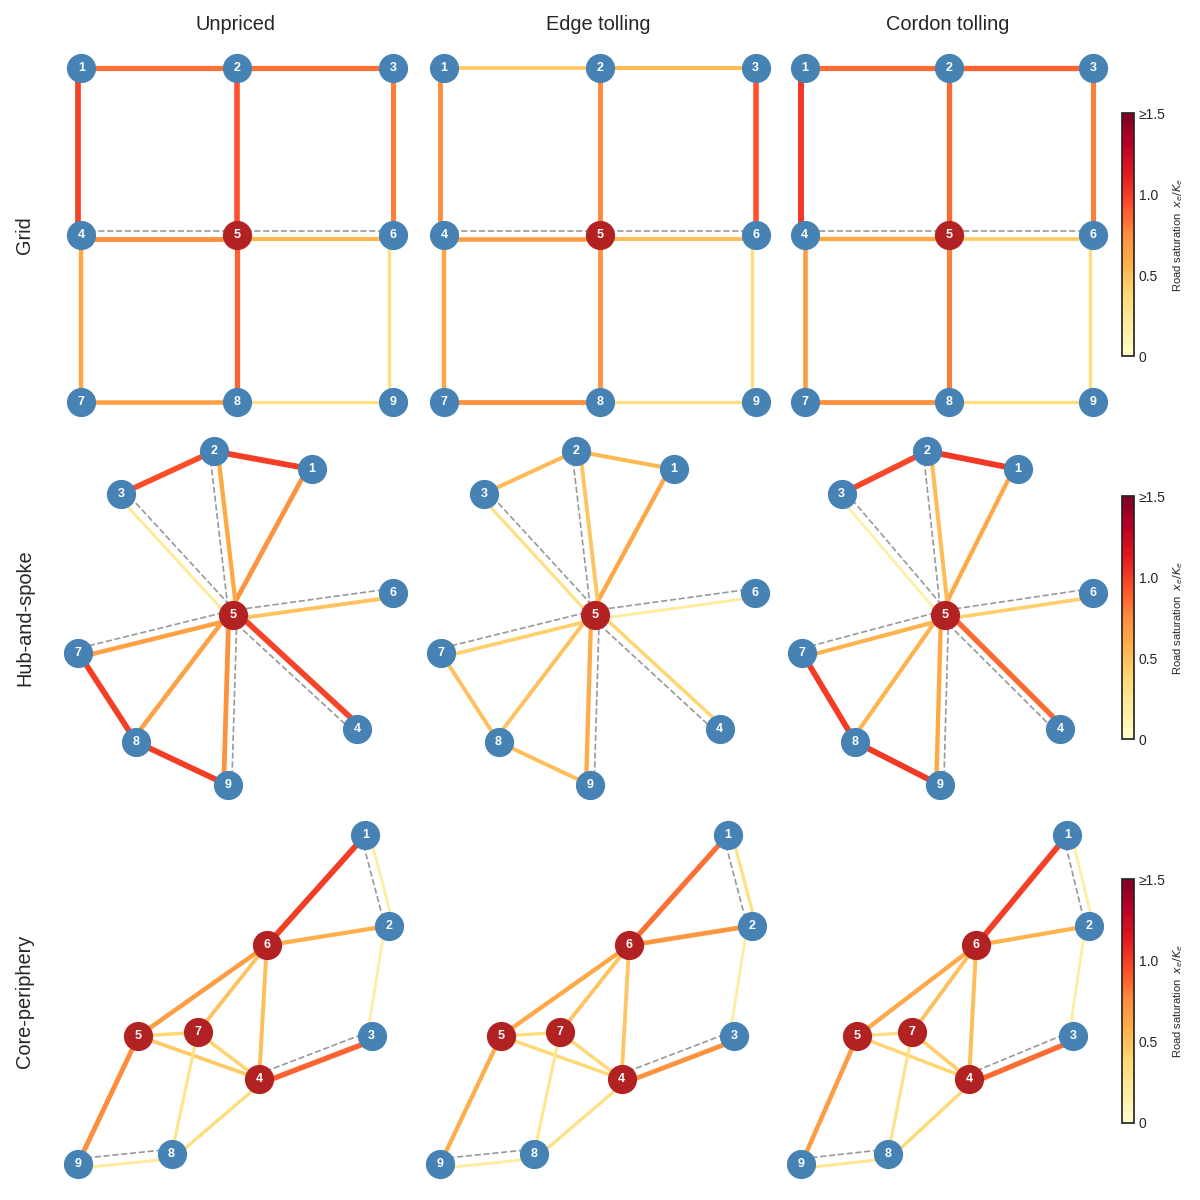
\includegraphics[width=\linewidth]{images/flow_maps.png}
    \caption{Heat maps of road edge saturation (the ratio of flow to capacity) in each network under each pricing regime.}
    \label{fig:flow_maps}
\end{figure}

\subsection{Sensitivity}

\Cref{tab:mode_shares_varying_theta,tab:tsc_varying_theta} report mode shares and TSC, respectively, when $\theta = 0.5$ and $\theta = 2$.
Recall that $\theta$ represents users' responsiveness to cost differences.
Low $\theta$ is relatively insensitive to such differences, high $\theta$ responds sharply to them.
This addresses how behavioral heterogeneity impacts the effectiveness of congestion pricing and mode shift.

Two patterns stand out.
First, at low $\theta$ the unpriced equilibrium TSC is higher; cost-insensitive travelers do not necessarily avoid congested routes.
The potential welfare gains from congestion pricing are accordingly larger, but cordon pricing performs poorly relative to first-best; the efficiency ratio falls below 0.23 across all networks.
A cordon toll is insufficient to shift behavior when travelers are already weakly responsive to cost signals.

Second, at high $\theta$ the cordon efficiency ratio becomes negative in all three networks.
The cordon TSC actually exceeds the unpriced TSC.
Highly cost-sensitive travelers respond aggressively to the toll by rerouting around the toll onto routes that were previously uncongested, inducing new congestion.
The effect is most severe in the grid with an efficiency ratio of \textminus 0.36, where a greater number of alternative routes makes such pricing ineffective on sensitive users.

\begin{table}
    \centering
    \footnotesize
    \begin{tabularx}{\textwidth}{l l R R R R}
    \toprule
    \textbf{Network} & \textbf{Pricing} & \multicolumn{2}{c}{\textbf{Car share}} & \multicolumn{2}{c}{\textbf{Transit share}} \\
    \cmidrule(lr){3-4} \cmidrule(lr){5-6}
    &  & $\theta = 0.5$ & $\theta = 2.0$ & $\theta = 0.5$ & $\theta = 2.0$ \\
    \midrule
    Grid            & Unpriced   & $0.8668$ & $0.6966$ & $0.1332$ & $0.3034$ \\
                    & First-best & $0.6569$ & $0.7335$ & $0.3431$ & $0.2665$ \\
                    & Cordon     & $0.8515$ & $0.6766$ & $0.1485$ & $0.3234$ \\
    \midrule
    Hub-and-spoke   & Unpriced   & $0.7199$ & $0.7222$ & $0.2801$ & $0.2778$ \\
                    & First-best & $0.3601$ & $0.4251$ & $0.6399$ & $0.5749$ \\
                    & Cordon     & $0.6741$ & $0.6435$ & $0.3259$ & $0.3565$ \\
    \midrule
    Core-periphery  & Unpriced   & $0.9105$ & $0.8278$ & $0.0895$ & $0.1722$ \\
                    & First-best & $0.8086$ & $0.8105$ & $0.1914$ & $0.1895$ \\
                    & Cordon     & $0.9022$ & $0.7940$ & $0.0978$ & $0.2060$ \\
    \bottomrule
\end{tabularx}
    \caption{Equilibrium mode shares under low and high $\theta$.}
    \label{tab:mode_shares_varying_theta}
\end{table}

\begin{table}
    \centering
    \footnotesize
    \begin{tabularx}{\textwidth}{l R R R r}
    \toprule
    \multicolumn{5}{c}{$\theta = 0.5$} \\
    \midrule
    \textbf{Network} & \multicolumn{3}{c}{\textbf{Total social cost}} & \textbf{First-best gap closed by cordon} \\
    \cmidrule(lr){2-4}
    & Unpriced & First-best & Cordon & \\
    \midrule
    Grid            & $542.6832$ & $469.3601$ & $540.2296$ & $0.0335$ \\
    Hub-and-spoke   & $735.2380$ & $647.0030$ & $715.0948$ & $0.2283$ \\
    Core-periphery  & $302.7127$ & $276.1063$ & $301.9440$ & $0.0289$ \\
    \bottomrule
\end{tabularx}
\begin{tabularx}{\textwidth}{l R R R r}
    \toprule
    \multicolumn{5}{c}{$\theta = 2.0$} \\
    \midrule
    \textbf{Network} & \multicolumn{3}{c}{\textbf{Total social cost}} & \textbf{First-best gap closed by cordon} \\
    \cmidrule(lr){2-4}
    & Unpriced & First-best & Cordon & \\
    \midrule
    Grid            & $473.4340$ & $484.3906$ & $469.4419$ & $-0.3644$ \\
    Hub-and-spoke   & $646.3785$ & $666.0452$ & $638.7758$ & $-0.3866$ \\
    Core-periphery  & $257.3444$ & $282.0954$ & $253.9962$ & $-0.1353$ \\
    \bottomrule
\end{tabularx}
    \caption{Total social cost under low and high $\theta$.}
    \label{tab:tsc_varying_theta}
\end{table}

\section{Discussion}

Cordon tolling performs well when the network topology aligns with the logic of its design.
The hub-and-spoke network is the clearest illustration of this.
Since virtually all cars routes funnel through the central hub, a cordon around that hub approximates the first-best instrument reasonably well, compared to the other networks; it recovers nearly 70\% of the first-best efficiency gain.
The core-periphery network behaves similarly for similar reasons.

The grid network exposes a core weakness of the cordon toll.
When travelers have many alternative routes of comparable cost, the toll does not eliminate congestion, rather it displaces it.
Travelers can effectively reroute around the cordon by car before having to switch to transit, so the toll simply redistributes flow.
So the 21\% efficiency ratio in the grid network is not necessarily evidence that cordon tolling is inherently ineffective.
Rather, it further demonstrates the importance of network topology, whether in regards to geography or urban layout, in designing a cordon.

Sensitivity to user behavior and preferences, captured in this model by $\theta$, is another important consideration.
Congestion pricing is not only generally less effective but can also produce negative welfare when travelers are highly sensitive to cost differences.
It can induce rerouting that distorts uncongested roads and worsens.
The social planner's solution, the first-best instrument, avoids this because it internalizes all flows simultaneously and optimizes them so that there is no untolled margin left for rerouting to exploit.
A real-world policy cannot do this.
Behavioral responsiveness is therefore something that must be understood and anticipated when designing congestion pricing policy.

We made several stylized decisions and simplifying assumptions to make this model tractable.
Chief among them is the fixed nature of transit.
Since one of the primary aims of many congestion pricing policies is to encourage people to drive less and use transit more, further work with this model should incorporate more realistic representation of transit.
Transit quality, congestibility, and multimodality, as well as people's preferences for cars over transit, are all things neglected in this model that have potential for future work.

\section{Conclusion}

We analyzed congestion pricing in a multimodal transportation network model that integrates route/mode choice and congestion externalities within a stochastic user equilibrium framework.
Using three stylized urban topologies, we found that the welfare effectiveness of cordon tolling as a congestion pricing policy is highly topology-dependent.
It can work well when the cordon coincides with a true network bottleneck but can be counterproductive when the network allows extensive rerouting or when travelers are highly sensitive to prices.

This should underscore the fact that there is no universal case for a congestion pricing policy independent of the network to which it is applied.
Cordon tolls are commonly discussed because they are administratively feasible, but practical implementations will be highly context dependent.
Our insights can be extended to future work with endogenous transit quality, heterogeneous traveler types, and joint optimization of cordon tolls and boundaries.

\setlength{\bibsep}{0pt}
\bibliographystyle{chicago}
\bibliography{report}

\end{document}
